\documentclass[preprint]{sigplanconf}

\usepackage[pdftex]{graphicx}
\usepackage[all]{xy}
\usepackage{tikz}
\usetikzlibrary{arrows, shapes, backgrounds, chains, decorations, calc, fit,
    shadows}
\usepackage[english]{babel}
\usepackage[Q=yes]{examplep}
\usepackage{pgf}
\usepackage{tikzuml-v1.0b/tikz-uml}
\usepackage{listings}

\lstset{
  basicstyle=\footnotesize\ttfamily
}

\begin{document}
\title{Bidirectional Git Objects Transferring by Subdirectories Specified}
\authorinfo{Congbin Guo\and Eric Wang}{VMware Inc.}{\{cguo,wange\}@vmware.com}
\maketitle
\abstract{
    \input abstract.input
}

\keywords
Git, transfer protocol, version control system, pack file, Git object model,
spare clone

\section{Introduction}
%(
% describe the problem
Git is popular but still has problems when work with large remote repositories,
which may consume lots of time and network bandwidth in data transferring from,
and to, the repository.
The reason is Git stores the history of whole workspace snapshots, which may
have huge amount of directories and files.
Many Git users has required the feature of transferring subdirectories, like
other popular version control systems do (e.g. Perforce), for long time.
But it is not in the plan of Git maintainers, because it may break Git
repository consistency and many other Git features\cite{roadmap}.
The suggestion from Git developers to deal with large repository is to break
into small ones, or omit some history by using Git shallow clone.
Neither one is very attractive to enterprise level users.

% my contribution
In this paper, we propose a solution to transfer subdirectories specified by
user from and to remote repositories efficiently.

\begin{itemize}
  \item We analyze the Git transfer protocol first, and extend it to allow
      subdirectories discovery and negotiation between server and client.

  \item Based on the extended protocol, we describe how to optimize the
      transferred data size to client by excluding some Git objects.

  \item More importantly, we discuss how to keep the newly created commits from
      the ``partial'' workspace as consistent as created from a full workspace.
\end{itemize}

%)
\section{Background}
\subsection{Git object model}
Git stores files, directories, and change histories as unique objects, i.e.
\emph{blob} \emph{tree} and \emph{commit}, with names derived from their SHA1
check sum value\cite{gitobj}.
It can be better explained by an example.
Figure \ref{fig:workspace} shows the two snapshots of an example workspace.
We modified \verb|file1| and \verb|file2|, and added a new file \verb|file4|.
\begin{figure}[htpb]
  \centering
  \input figures/workspace.tikz
  \caption{Snapshots of the example workspace}
  \label{fig:workspace}
\end{figure}

Figure \ref{fig:git-repo} shows the repository.
Accordingly, there are two commit objects, $C$ and $C'$, with tip $H$ pointing
to the current version, i.e. \verb|HEAD|.
Because \verb|file3| is unchanged, the two commits share blob $B_3$.

\begin{figure}[htpb]
  \centering
  \begin{tikzpicture}[node distance=1.5cm, every node/.style={align=center}]
\input figures/git-model-base.tikz
\end{tikzpicture}

  \caption{Git repository for an example workspace}
  \label{fig:git-repo}
\end{figure}

\subsection{Git Transfer Protocol}
%(
Current Git transfer protocol is simple and clear\cite{tran-protocol}.
Figure \ref{fig:git-proto-clone-seq} shows the steps of transferring data from
server, i.e. cloning or fetching.

\begin{enumerate}
  \item Client initiates the request by calling \verb|git-upload-pack| on
    server.

  \item Server advertises all current reference SHA1s ($H_s$) to the client.

  \item Client sends a list of SHA1 of \verb|want| ($H_w$) and \verb|have|
    ($H_h$), which indicates the start and end SHA1 of commit objects to be
    transferred.
    In case of cloning, the list of \verb|have| is skipped since the client has
    nothing yet.

  \item Server calculates all commit objects (and all other Git objects
    associated) in range of $[H_w, H_h)$, then writes to a stream connected to
    the client.
\end{enumerate}

\begin{figure}[htpb]
  \centering
  %!tikz editor 1.0
%!tikz source begin
\begin{tikzpicture}
\begin{umlseqdiag}
\umlobject[class=Client]{c}
\umlobject[class=Server]{s}
\begin{umlcall}[op={git-upload-pack}]{c}{s}
  \begin{umlcall}[op={$H_s$}, type=return]{s}{c}
  \end{umlcall}
  \begin{umlcall}[op={$<H_w, H_h>$}, return={pack stream}]{c}{s}
    \begin{umlcall}[op={pack-objs}]{s}{s}
    \end{umlcall}
  \end{umlcall}
\end{umlcall}
\end{umlseqdiag}
\end{tikzpicture}
%!tikz source end


  \caption{Transferring Git objects from server}
  \label{fig:git-proto-clone-seq}
\end{figure}
The Git transfer protocol also covers the opposite direction, i.e. transfer
data from client to server, i.e.\emph{push}.
Because it is fully reused in our solution, we do not describe it in detail
here.

\section{The problem}
To support subdirectories transferring between server and client needs to
resolve below problems:
\begin{itemize}
  \item How does the client discovery the subdirectories, and negotiate with
      the server that which of them to be transferred?

  \item How does the server optimize the Git objects pack according to chosen
      subdirectories?

  \item How does the client operate with the partial Git objects store, and
      furthermore ensure the newly created commits are as good as the ones
      from fully Git objects store?
\end{itemize}
%)

\section{Solution}
Our solution includes both server side and client side changes.
\subsection{Server side}
We add two more steps in server side, one is negotiating subdirectories,
and another is excluding uninterested objects from packing.
\subsubsection{Subdirectories Negotiation}
Client can send all subdirectories interested and excluded when it has enough
information.
Otherwise, the negotiation is necessary.
The subdirectories negotiation is an interactive process because the client may
know nothing about the directories, especially in cloning.

We add an extra step in the standard transfer protocol to allow subdirectories
negotiation between client and server.
The step is initiated by client, so it is transparent for common Git client,
which can ensure the server compatibility for all kinds of client.
\begin{figure}[htpb]
  \centering
  %!tikz editor 1.0
%!tikz source begin
\begin{tikzpicture}
\begin{umlseqdiag}                                                             
\umlobject[class=Client]{c}                                                    
\umlobject[class=Server]{s}                                                    
\begin{umlcall}[op={git-upload-pack}, return={pack stream}]{c}{s}
    \begin{umlcall}[op={$H_S$}, type=return]{s}{c}
    \end{umlcall} 
    \begin{umlfragment}[type=loop]
        \begin{umlcall}[op={dir}]{c}{s}
        \end{umlcall}
        \begin{umlcall}[op={$D_S$}, type=return]{s}{c}
        \end{umlcall}
    \end{umlfragment}
    \begin{umlcall}[op={$<H_h, H_w, D_i, D_e>$}]{c}{s}
    \end{umlcall}
    \begin{umlcall}[op={pack_objs($[H_s, H_c), D_i, D_e$)}]{s}{s}
    \end{umlcall}                 
\end{umlcall}  
\end{umlseqdiag}
\end{tikzpicture}
%!tikz source end


  \caption{Extended Git transfer protocol}
  \label{fig:git-proto-ext-seq}
\end{figure}

By following the style in \cite{tran-protocol}, we define the extended
protocol command in ABNF as well, which shown in Figure
\ref{fig:git-proto-ext-ABNF}.
The extension includes three primitive commands.
\begin{itemize}
  \item \verb|dir| get a list of files and directories under \verb|path| of a
    \verb|SHA1|, which equivalent to what command
    \verb|git ls-tree SHA1 -- path| does.

  \item \verb|include| specify files or subdirectories to be included in data
    transferring.

  \item \verb|exclude| specify files or subdirectories to be excluded from data
    transferring.
\end{itemize}

\begin{figure}[htpb]
  \centering
  \begin{verbatim}
  upload-request = dir-commands
                   want-list
                   have-list
                   dir-requests
                   compute-end

  dir-commands = *dir-command

  dir-command = PKT-LINE(dir SP obj-id SP path LF)

  dir-requests = *(dir-request)

  dir-request = include-line | exclude-line

  include-line = PKT-LINE(include SP path LF)

  exclude-line = PKT-LINE(exclude SP path LF)
  \end{verbatim}
  \caption{ABNF of extended Git transfer protocol}
  \label{fig:git-proto-ext-ABNF}
\end{figure}

We define the server response of \verb|dir| command in ABNF as well, as shown
in Figure \ref{fig:server-response-ABNF}.
It follows the output format of command \verb|git ls-tree|, which we reuse to
help create the response.
\begin{figure}[htpb]
  \centering
  \begin{verbatim}
  advertised-dirs = dir-list
                    flush-pkt

  dir-list = *(dir-line)

  dir-line = PKT-LINE(mode SP type SP obj-id \
                      TAB name LF)

  type = tree | blob
  \end{verbatim}
  \caption{ABNF of server response}
  \label{fig:server-response-ABNF}
\end{figure}

In the example repository shown in Figure \ref{fig:git-repo}, supposing the
client only want \verb|file1|, the subdirectories discovery and negotiation may
look like what shown in Figure \ref{fig:c/s-comm}.
All lines asterisked are the extension proposed.

\begin{figure}[htpb]
  \centering
  \begin{verbatim}
    S: 00887217a7c...ba0 HEAD\0multi_ack\
       thin-pack side-band side-band-64k\
       ofs-delta shallow no-progress include-tag
    S: 003f7217a7c...ba0 refs/heads/master
    S: 0000
  * C: 002fdir 7217a7c...ba0 /\n
  * C: 0000
  * S: 003b040000 tree 0760d56...353\t/dir1\n
  * S: 003c100644 blob 3176af7...989\t/file1\n
  * S: 003c100644 blob 1270084...e27\t/file4\n
  * S: 0000
    C: 0054want 7217a7c...ba0\0multi_ack \
       side-band-64k ofs-delta\n
    C: 0000
    C: 0032have 5a3f6be...b68a\n
    C: 0000
  * C: 000ainclude /\n
  * C: 000fexclude /file4\n
  * C: 000eexclude /dir1\n
  * C: 0000
    C: 0009done\n
  \end{verbatim}
  \caption{Server/Client communication example}
  \label{fig:c/s-comm}
\end{figure}

\subsubsection{Objects Packing Optimization}
In standard Git protocol, the object packing can be regards as a piped command,
i.e.
\begin{verbatim}
git-rev-list|git-pack-objects
\end{verbatim}
That is, get a list of all commits (and its associated objects) first, and then
pack them.

To save time and network bandwidth to transfer, we reduce the amount of objects
by finding out ones can be removed.
\begin{itemize}
  \item We keep tag objects because they have minor impact to repository size.

  \item We keep commit objects because they are the backbone of the repository
    and ensure the consistency.

  \item We remove blob and tree objects in case the files or directories they
    represent are not in the subdirectories specified.

\end{itemize}

In the example repository shown in Figure \ref{fig:git-repo}, still supposing
the client only wants \verb|file1| (represented as $B_1$ and $B'_1$), the
candidate objects for excluding are tree objects ($T_1$ and $T'_1$), and blob
objects ($B_2$, $B'_2$, $B_3$ and $B_4$), as highlighted in Figure
\ref{fig:find-obj-to-remove}.
After that, we have a reduced object list, and then pass it to
\verb|git-pack-objects| command to pack.
\begin{figure}[htpb]
  \centering
  \begin{tikzpicture}[node distance=1.5cm, every node/.style={align=center}]
\input figures/git-model-base.input
\begin{pgfonlayer}{background}
  \node[ellipse, fill=black!20, fit=(tr1_1) (b1_2) (b1_3), xscale=0.75,
  yshift=-0.5cm]{};
  \node[ellipse, fill=black!20, fit=(tr2_1) (b2_2) (b2_4)]{};
\end{pgfonlayer}
\end{tikzpicture}

  \caption{Objects can be excluded in the example repository}
  \label{fig:find-obj-to-remove}
\end{figure}


\subsection{Client side}
\subsubsection{Packed Objects Receiving}
The client cannot handle the pack stream transferred from server directly
due to the excluded objects.
We create placeholder files in client for the excluded ones.
We call those placeholders \emph{Git mock objects}.
The mock objects have same name, i.e. the SHA1 string of the object, as the
original objects.
But the content of mock objects is empty.

The reason why we can use empty file as the placeholder is because that Git
performs consistency checks based on SHA1 values got from the object file name,
rather than re-calculate it again from the content.
In other words, Git only cares about the object file name instead of the
content.

Figure \ref{fig:cmd-create-mock} shows one way to create empty blob and tree
object by command line.
The object file prefixed with \verb|e69de29| and \verb|4b825dc| are the mock
blob and tree object we want.
They can play the placeholder to any same type Git object by just renaming it
to target SHA1.
The benefits of using those mock objects are:
\begin{enumerate}
  \item They are still Git objects with correct format, though named with SHA1
    string of another object.

  \item The cost to create them is very low because of the small file size.

  \item An empty tree object dereferences all associated objects;
    so eliminates the need for placeholders for all sub-trees and blobs.
\end{enumerate}


\begin{figure}[htpb]
  \centering
  \begin{verbatim}
    # create an empty blob object
    $ :> empty_file
    $ git hash-object -w empty_file
    e69de29bb2d1d6434b8b29ae775ad8c2e48c5391

    # create an empty tree object
    $ git mktree <<EOF
    EOF
    4b825dc642cb6eb9a060e54bf8d69288fbee4904
  \end{verbatim}
  \caption{Command line to create Git mock objects}
  \label{fig:cmd-create-mock}
\end{figure}

Figure \ref{fig:mock-objects} shows the resulting diagram with the mock
objects.

\begin{itemize}
  \item The mock object $B_m$ replaces the blob object $B_4$.

  \item The mock tree object $T_m$ and $T'_m$ replace two tree objects, $T_2$
    and $T'_2$.
\end{itemize}

\begin{figure}[htpb]
  \centering
  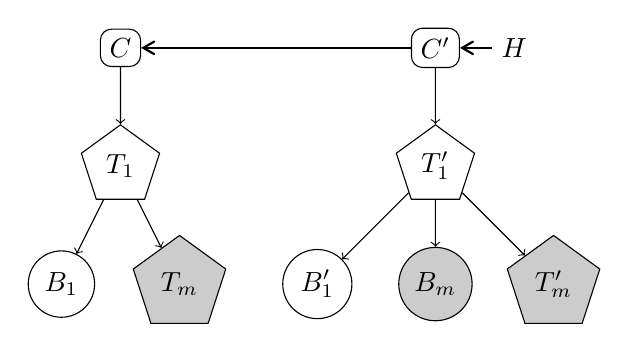
\begin{tikzpicture}
\tikzstyle{commit}=[rectangle, draw, rounded corners]
\tikzstyle{tree}=[regular polygon, regular polygon sides=5, draw, thin]
\tikzstyle{blob}=[circle, draw, thin]

% mock tree/blob object
\tikzstyle{mock_tree}=[regular polygon, regular polygon sides=5, draw, thin,
  fill=black!20]
\tikzstyle{mock_blob}=[circle, draw, thin, fill=black!20]

\tikzstyle{parent}=[-angle 60, draw, thick]
\tikzstyle{edge from parent}=[->, draw]
\tikzstyle{2obj}=[->, draw]
% tree 1
\node[commit](ci1){$C$}
child{node[tree](tr1){$T_1$}
  child{node[blob](b1_1){$B_1$}}
  child{node[mock_tree](tr1_1){$T_m$}}
};

% tree 2
\node[commit, right of=ci1, node distance=4cm](ci2){$C'$}
child{node[tree](tr2){$T'_1$}
  child{node[blob](b2_1){$B'_1$}}
  child{node[mock_blob](b2_4){$B_m$}}
  child{node[mock_tree](tr1_1){$T'_m$}}
};

\draw[parent](ci2) to (ci1);


% HEAD
\node[rectangle, right of=ci2](head){$H$};
\draw[parent](head) to (ci2);


\end{tikzpicture}

  \caption{Replacing Git objects with mock objects}
  \label{fig:mock-objects}
\end{figure}

With those mock objects, Git is happy with the data transferred from server.

\subsubsection{Workspace Checking-out}
Like normal Git objects, Git can also check out the mock objects into workspace.
The checked-out mock blob objects is an empty file.
And the checked-out mock tree object is nothing.

The checking out of those mock objects can make Git regards the current
workspace is dirty.
That is because Git recalculates the SHA1 value of working files and compare
what recorded in Git index.
Obviously, they are different.

We use \emph{Git sparse checkout} \cite{sparseco} to avoid that, which only
checkout specified subdirectories from repository into workspace.
Here we can reuse the result of subdirectories negotiation done before.
That is what user exactly wants to get initially.



\subsubsection{New Commits Creating}\label{sec:create-new-commit}
Git staging area, or \emph{index}, which generally kept in \verb|.git/index|,
is the key data structure for Git to prepare a new commit.
It contains a sorted list of all path names of current tree, each with
permissions and the SHA1 of a blob object \cite{idx-format}.
Git uses the data stored in index to create a tree object; then creates a
commit with that tree.
Even for Git sparse checking out, in which only a part of files be checked
out, the index still contains a full list of all files for committing.

In our case, Git index loads nothing by reading mock tree objects
since they are empty.
This results in partial Git index which cannot work properly when creating new
commits, because Git index regards all directories represented by mock tree
objects as removed.

It makes no sense for users to modify files out of the scope of
subdirectories negotiated in our solution.
Based on that, we extract missing blob and tree objects information from the
most recent commit; combine it with data stored in the Git index to form a
complete tree object; and then rewrite the commit to point to the complete tree
object.
We do the rewriting just after every new commit created.
Below is the more detail steps:

\begin{enumerate}
  \item Get the tree object content of current version $T_h$, i.e. \\
        \verb|git cat-file -p HEAD^{tree}|.

  \item Get staging files path and SHA1 information $T_t$ from Git index.

  \item Combine the content of $T_h$ and $T_t$ together; and then construct a
        new tree object $T$ by command \verb|git mktree|.

  \item Run command \verb|git commit-tree |$T$ to create a new commit object
        $C$.

  \item Update current branch tip to pointed to $C$ by command \\
        \verb|git update-ref|.
\end{enumerate}

\section{The details}
\subsection{System Implementation}
We developed a prototype to prove the solution works.
Figure \ref{fig:components} shows the system level components interaction.
The key components for the proposed solution includes:
\begin{itemize}
  \item \emph{Subdirs} communicates with client to track which subdirectories
    of the repository to be transferred.

  \item \emph{Filter} gets the objects list from
    \verb|git rev-list| command, and filters them by subdirectories specified.
    The component has two outputs.
    One is \emph{real object list} that passes to object-packing component.
    Another is \emph{mock object list}, which is a subset of filtered out
    objects, passes to \emph{mock object builder} on client.

  \item \emph{Mock object builder} accepts the mock object list
    from the filter, and then create mock objects accordingly.
    It builds the mock objects in pack file format\cite{packformat} for better
    performance.

  \item \emph{Commit creator} creates new commits and ensures
    the tree object of commit is complete as described in Section
    \ref{sec:create-new-commit}.
\end{itemize}
\begin{figure}[htpb]
  \centering
  \usetikzlibrary{shapes, shadows, fit, arrows, positioning}
\tikzstyle{object} = [draw, rectangle, rounded corners, align=center, minimum
height=1cm]
\tikzstyle{new} = [fill=black!20]
\tikzstyle{pack} = [object, minimum width=35mm]
\tikzstyle{comp} = [draw, rectangle, minimum height=1cm, minimum width=0.6cm,
  very thick]
\tikzstyle{filter} = [draw, diamond, very thick]
\tikzstyle{view} = [draw, tape, tape bend top=none, double copy shadow, fill=white, minimum
height=1cm, minimum width=0.6cm, very thick]
\tikzstyle{box} = [rectangle]
\tikzstyle{network} = [draw, cloud, cloud puffs=61, fill=white, minimum width=7cm]
\tikzstyle{olist} = [->, thin, sloped]
\tikzstyle{consume} = [single arrow, midway, draw, sloped, align=center,
  minimum height=5mm, single arrow head extend=1mm]
\tikzstyle{stream} = [single arrow, draw, sloped, minimum height=3mm, single
  arrow head indent=1mm, single arrow head extend=2mm]
\tikzstyle{stream2} = [stream] %, shape border rotate=180]
\tikzstyle{vlabel} = [anchor=south, rotate=-90]

\ifdefined\PRETTY
  \tikzset{object/.append style={top color=black!20, draw=black!30, drop
      shadow, text=black!80}}
  \tikzset{new/.append style={top color=white, middle color=yellow!50!red,
     drop shadow, draw=red!50, text=red!50!black}}
  \tikzset{network/.append style={bottom color=gray, top color=white,
      drop shadow, draw=black!60, text=blue!50!black}}
  \tikzset{comp/.append style={drop shadow, fill=blue!20, draw=blue!10,
      text=blue!40!black!50}}
  \tikzset{stream/.append style={drop shadow, top color=green!30,
      draw=green!50}}
  \tikzset{consume/.append style={drop shadow, fill=yellow!50!red,
      draw=yellow}}
  \tikzset{vlabel/.append style={font=\large\scshape, text=black!60}}
\fi

\begin{tikzpicture}
  \node[matrix, label={above:Server Repository}, column sep=2mm](repo)
  {
    \node[object](obj1){loose\\object}; &
    \node[object](obj2){loose\\object}; &
    \node[pack, minimum width=45mm](obj4){pack file}; \\
  };

  \node[comp, below=1cm of repo.west, anchor=north west](revlist){\verb|git|\\\verb|rev-list --all --objects|};
  \node[filter, new, below of=revlist, node distance=1.5cm](f){filter};
  \node[view, new, anchor=west](v) at(revlist.west |- f){subdirs};
  \node[comp, below =3.5cm of revlist.east, anchor=east](gitpack){Git object packing};
  \node[box, fit= (gitpack)(repo)](server){};
  \node[vlabel, anchor=north] at (server.east){Server};

  % client side
  \node[pack, below= 3.2cm of gitpack](pack){pack file};
  \node[object, left = 2mm of pack.west, anchor=east](mockobj){mock\\objects};
  \node[object, right=2mm of pack.east, anchor=west](newobj){new\\commits};
  \node[comp, new, below =5mm of newobj](ci-ctor) {Commit\\Creator};
  \node (x) at (obj4.south-|newobj){};
  \path(newobj) to node[stream2, minimum height=8cm, pos=.48]{git push}(x);
  \node[comp, new, above=5mm of mockobj](mockc){Mock object\\builder};
  \node[comp, anchor=west, minimum width=45mm] (idx) at (mockobj.west |- ci-ctor) {Git \emph{Index}};
  \draw[olist] (idx) -- (ci-ctor);
  \draw[olist] (pack) -- (ci-ctor);
  \path(ci-ctor) to node[stream]{} (newobj);

  \node[box, fit=(mockc)(ci-ctor)](c){};
  \node[vlabel] at (c.east) {Client};
  \draw[thick](repo.south east) -- (repo.south west);

  \path(v) to node[consume, minimum width=3mm]{} (f);
  \draw[olist](obj1.south) -- (revlist);
  \draw[olist](obj2.south) -- (revlist);
  \draw[olist](obj4.south) -- (revlist);
  \draw[olist](revlist) -- (f);

  \draw[olist](f) to node{real obj\\list} (gitpack);
  \draw[olist](f) to [in=90, out=-140] node[near start]{mock obj\\list} (mockc);
  \path(gitpack) to node[stream2, minimum height=30mm, pos=.5, label={[above]45:git fetch}]{}
     node [network, aspect=3, pos=.3]{Network} (pack);
  \path(mockc) to node[stream] {} (mockobj);
%  \node[draw, single arrow, minimum height=3cm, align=left, text justified] at (0, 0){test\\1};
\end{tikzpicture}

  \caption{System level components}
  \label{fig:components}
\end{figure}

\subsection{Example Work flow}
We implemented a new git remote helper\cite{git-remote-helper} for the proposed
protocol extension.
The remote helper provides a new remote repository URL scheme \emph{dirs://}.
By replacing normal \emph{ssh://} scheme with that, the helper calls the
extended protocol automatically.
The repository we used is a Git mirror of a perforce depot, i.e.\\
\verb|mirrors/vmware/perforce-1666_bora_prod-2015.git| from
\verb|git.eng.vmware.com|, which size is about 3.0GB.

First, we created an initial clone.
\begin{verbatim}
$ git clone
dirs://cguo@cguo-dev2.eng.vmware.com/build/mts/tmp/\
     mirrors/vmware/perforce-1666_bora_prod-2015.git
Cloning into 'perforce-1666_bora_prod-2015'...
INFO:root:Calling editor...
\end{verbatim}
The prototype popped up an editor to show the top level directories of the
repository with usage, e.g.
\begin{verbatim}
# Git repo cguo@cguo-dev2.eng.vmware.com/build/mts/\
  tmp/mirrors/vmware/perforce-1666_bora_prod-2015.git
# Below is the top level file structure of the repo.
# Please comment out the files/directories you want.
# This file has same syntax with '.gitignore'.

#/bora-vmsoft
#/bora
#/mojo
#/scons
#/vmkdrivers
\end{verbatim}

For example, we only comment out directory \verb|/scons|.
After saving and exiting the editor, the program starts the transferring.
\begin{verbatim}
remote: = Extended version of git-pack-objects =
remote: = Transferring by subdirectories =
remote: Counting objects: 52510, done.
...
\end{verbatim}

We did another normal cloning for comparing.
\begin{verbatim}
$ git clone
ssh://cguo@cguo-dev2/build/mts/tmp/\
    mirrors/vmware/perforce-1666_bora_prod-2015.git
Cloning into 'perforce-1666_bora_prod-2015'...
remote: = Extended version of git-pack-objects =
remote: = Normal git clone =
remote: Counting objects: 505844, done.
...
\end{verbatim}
The total objects transferred reduced from 505,844 to 52,510 (about 90\%
reduced!).
The objects size transferred also reduced from 3.0GB to 24MB (about 99\%
reduced!).

Finally, we created a new commit by adding a \verb|readme| file to \verb|scons/|
directory.
\begin{verbatim}
$ echo This is a test > scons/readme
$ git add scons/readme
$ git commit -am \
      'Subdirectories transferring is awesome!'
= Commit rewritten to b72f3ee =
[master e1dfc03] Subdirectories transferring is awesome!
 1 file changed, 1 insertion(+)
  create mode 100644 scons/readme
\end{verbatim}
From above output, we saw the new commit created is \verb|b72f3ee| instead of
\verb|e1dfc03|.
We ran below commands to verify the newly created commit is correct.
\begin{verbatim}
$ git ls-tree e1dfc03
040000 tree 90d69f5...7c1    scons
$ git ls-tree b72f3ee
040000 tree fc6b587...6d5    bora-vmsoft
040000 tree d850081...68b    bora
040000 tree 41b08a1...c43    mojo
040000 tree 90d69f5...7c1    scons
040000 tree 33c7dc2...344    vmkdrivers
\end{verbatim}
That is, the tree of rewritten commit \verb|b72f3ee| includes both
the subdirectory we transferred, and others we filtered out.

After pushing the newly created commit back to remote, we finished the
example work flow.

\section{Related work}
E. Newren did some inspiring work in \cite{newren10-0}, \cite{newren10-1},
which describes the idea of just clone referenced objects to client side.
Additionally, this work also uses \emph{git replace} mechanism to deal with
commit history\cite{git-replace}.
However, due to modification to cloned commits and index file, some common Git
important operations cannot work perfectly, such as fetch, push, rebase, etc.

N. Duy has also begun to work on sparse clone or subtree clone since 2008; and
who submitted a series of patch in Git community.
\cite{duy08}, \cite{duy10-1}, \cite{duy10-2}, and \cite{duy10-3} describes a
sparse clone method by adding an extra option to \verb|git clone| command, and
rewriting/replacing the commits in clone time.
The work also has pointed out the performance limitation of Git replacement
mechanism.
The weak part of the work is multiple directories cannot be fully supported.

\section{Limitations}
Because of changing in Git object store, the client side repository cannot
support any Git operations care about repository, e.g. the command of
\verb|fsck|, \verb|repack|, and \verb|gc|.
Additionally, since the mock tree object is empty, running the command of
\verb|ls-tree| or \verb|cat-file| on that tree object produces empty output.

Another limitation is, since the Git index is partial comparing with normal Git
workspace, commands related to Git index (e.g. \verb|git ls-files|) may give
different results.

\begin{thebibliography}{10}
    \softraggedright

    \bibitem{roadmap} J. Hamano (July 2008).
    \newblock \emph{sparse fetch}.
    \newblock Git mailing list.
    \newblock URL
    [http://thread.gmane.org/gmane.comp.version-control.git/89681/focus=90016]

    \bibitem{gitobj} S. Chacon (July 2009).
    \newblock\emph{Pro Git}, section 9.2.
    \newblock URL
    [http://git-scm.com/book/en/Git-Internals-Git-Objects].

    \bibitem{tran-protocol} \emph{Pack files transfer protocol}.
    \newblock URL
    [https://www.kernel.org/pub/software/scm/git/docs/v1.7.0.5/\\
      technical/pack-protocol.txt].

    \bibitem{sparseco} \emph{Git-read-tree(1) Manual Page} (February 2013).
    \newblock URL
    [https://www.kernel.org/pub/software/scm/git/docs/git-read-tree.html]

    \bibitem{idx-format} \emph{GIT index format}.
    \newblock URL
    [https://www.kernel.org/pub/software/scm/git/docs/technical/\\
    index-format.txt].

    \bibitem{packformat} \emph{GIT pack format}.
    \newblock URL
    [https://www.kernel.org/pub/software/scm/git/docs/technical/\\
    pack-format.txt].

    \bibitem{git-remote-helper} \emph{git-remote-helpers(1) Manual Page}
        (February 2013).
    \newblock URL
    [https://www.kernel.org/pub/software/scm/git/docs/git-remote-helpers.html].

    \bibitem{newren10-0}E. Newren (July 2010).
    \newblock \emph{Sparse clones}.
    \newblock Git mailing list.
    \newblock URL
    [http://article.gmane.org/gmane.comp.version-control.git/152020].

    \bibitem{newren10-1}E. Newren (September 2010).
    \newblock \emph{Sparse clones}.
    \newblock Git mailing list.
    \newblock URL
    [http://article.gmane.org/gmane.comp.version-control.git/155389].

    \bibitem{git-replace} \emph{git-replace(1) Manual Page} (February 2013).
    \newblock URL
    [https://www.kernel.org/pub/software/scm/git/docs/git-replace.html].

    \bibitem{duy08}N. Duy (July 2008).
    \newblock \emph{git-clone: support --path to do sparse clone}.
    \newblock Git mailing list.
    \newblock URL
    [http://article.gmane.org/gmane.comp.version-control.git/89681].

    \bibitem{duy10-1}N. Duy (July 2010).
    \newblock \emph{Subtree clone?}.
    \newblock Git mailing list.
    \newblock URL
    [http://article.gmane.org/gmane.comp.version-control.git/151937].

    \bibitem{duy10-2}N. Duy (July 2010).
    \newblock \emph{Subtree clone proof of concept}.
    \newblock Git mailing list.
    \newblock URL
    [http://article.gmane.org/gmane.comp.version-control.git/152347].

    \bibitem{duy10-3}N. Duy (August 2010).
    \newblock \emph{subtree clone v2}.
    \newblock Git mailing list.
    \newblock URL
    [http://article.gmane.org/gmane.comp.version-control.git/154343].

\end{thebibliography}

\end{document}

